\documentclass[a4paper,11pt]{article}
\usepackage[T1]{fontenc}
\usepackage[utf8]{inputenc}
\usepackage{lmodern}
\usepackage[pdftex]{graphicx}

\title{Beam Switching}
\author{Tom Kuiper}

\begin{document}

\maketitle
\tableofcontents

\begin{abstract}
This is a tentative analysis of beam switching based on data for DSS-63, 
pending the data for DSS-43.

Differencing the signals from two feeds can remove the effect of a fluctuating 
atmospheric brightness temperature. Any gain difference between the two signal 
paths, however, will register as an apparent continuum with the spectral 
signature of the gain difference.  

Switching the source from one feed to the other and combining
those spectra removes this undesirable effect, but only to the extent that the
gain is stable between the two measurements.

Differences in gain between the two paths can be reduced by averaging them,
alternating the receivers with respect to the front end channels.

Normalized spectra are commonly used in spectral line reduction software.  They
may not be the best for canceling baseline effects, though.
\end{abstract}

\section{Raw Spectra}

\subsection{Feed Differencing}

With feed~1 pointing at the source, the powers registered by receivers~A and~B
and their difference are
\begin{eqnarray}
P_A &=& G_1 G_A ( T_{rec} + T_{sky} + T_{src} ) \nonumber \\
P_B &=& G_2 G_B ( T_{rec} + T_{sky} ) \nonumber \\
P_1 &=& P_A - P_B \nonumber \\
    &=& G_1 G_A T_{src} + (G_1 G_A - G_2 G_B)(T_{rec} + T_{sky}) \label{eqn:src-fd1}
\end{eqnarray}
where $G_1$ and $G_2$ are the time-averaged gains of the amplifiers of the
front end channels, and $G_A$ and $G_B$ are the time-averaged gains of 
receiver~A and receiver~B. $T_{sky}$ is the same for both feeds so it cancels 
even though it fluctuates, at least to the extent that $G_1 G_A = G_2 G_B$. 
 
This procedure is equivalent to {\it chopping} except that different signal
paths are used to measure the source and the reference.
To the extent that $G_1 G_A \ne G_2 G_B$, 
there is incomplete cancellation and the spectrum baseline will have the 
spectral signature of this difference.
Figure~\ref{fig:DSS63gains} shows the gains of the cryogenic K-band 
amplifiers on DSS-63.
\begin{figure}[h!tb]
  \begin{center}
    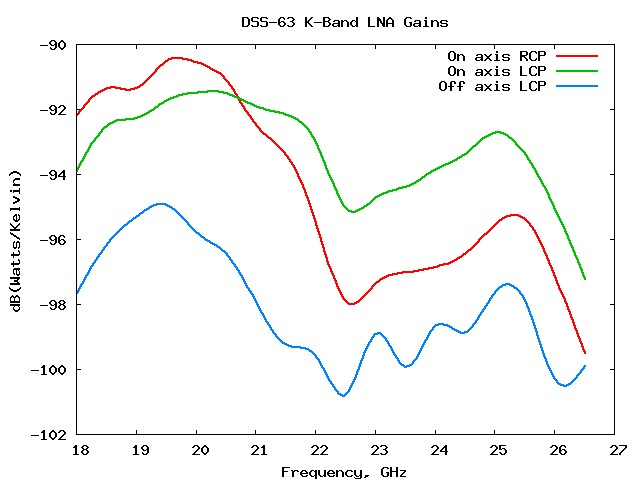
\includegraphics[width=4in]{DSS-63_gains.jpg}
    \caption{\label{fig:DSS63gains}Gains of the cryogenic K-band amplifiers
    on DSS-63. (Data provided by Manuel Franco.)}
  \end{center}
\end{figure}
Taking the data for DSS-43, the LCP channels for both DSS-63 ``on-axis''
feeds differ by about 5 dB.  Thus, the difference in the power between the 
two channels si about of factor of 3, which means that the difference
spectrum will have an apparent continuum of twice the off-axis power or
2/3 of the on-axis power, with the difference of spectral signatures of the
two channels.

There is considerable variation with frequency.  Even if 4.9~dB of attenuation
were inserted in the LCP path, Figure~\ref{fig:gain-diff} shows that there 
would be differences as large as 2~dB (-47 to + 58\%).
\begin{figure}[h!tb]
  \begin{center}
    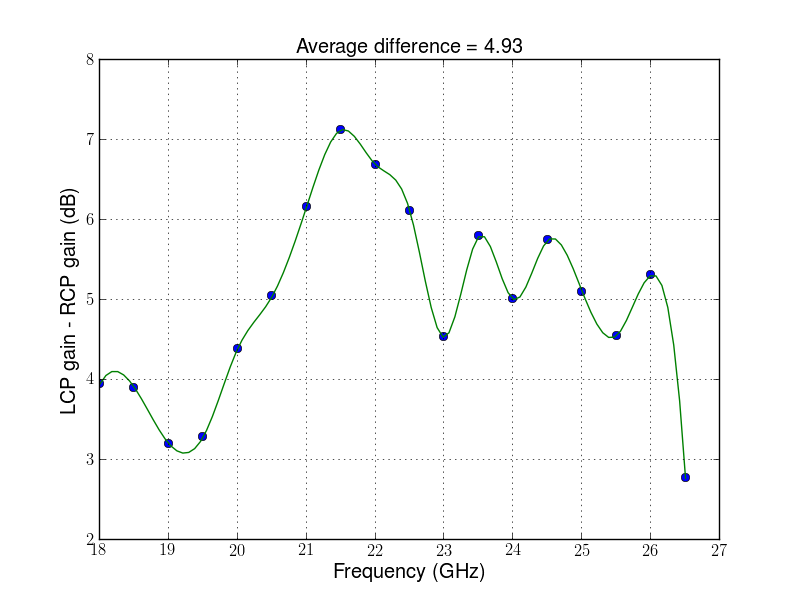
\includegraphics[width=4in]{gain_diff.png}
    \caption{\label{fig:gain-diff}Difference in gain between the K-band LCP
    ``on-axis'' and ``off-axis'' feeds.}
  \end{center}
\end{figure}

Also, if the source emission has a continuum as well as spectral lines, the
continuum will have the false spectral signature of $(G_1 G_A - G_2 G_B)$.

\subsection{Beam Switching}

With feed~2 pointing at the source,
\begin{eqnarray*}
P_A &=& G_1 G_A ( T_{rec} + T_{sky}) \nonumber \\
P_B &=& G_2 G_B ( T_{rec} + T_{sky} + T_{src} ) \nonumber \\
P_2 &=& P_B - P_A \nonumber \\
    &=&  G_2 G_B T_{src} + (G_2 G_B - G_1 G_A)(T_{rec} + T_{sky}) \label{eqn:src-fd2}
\end{eqnarray*}
This should have the same baseline spectral signature as $P_1$, but inverted,
if the gains are stable during the measurements of $P_1$ and $P_2$.

Adding the two measurements cancels the baselines.
\begin{eqnarray}
2 P_{src} &=& P_1 + P_2 \nonumber \\
          &=& (G_1 G_A + G_2 G_B) T_{src} \label{eq:pos1}
\end{eqnarray}
To the extent that the gains are not stable, the cancellation is incomplete and
will result in a spectrally varying pseudo-continuum or ``bad baseline''.

This is equivalent to telescope {\it nodding} although, since the two feeds are
almost horizontal, perhaps {\it wagging} would be a better term.

\subsection{Feed Switching}\label{sec:feedsw}

With the receivers switched with respect to the feeds and feed 2 pointing at 
the source,
\begin{eqnarray*}
P_A &=& G_2 G_A ( T_{rec} + T_{sky} + T_{src} )\\
P_B &=& G_1 G_B ( T_{rec} + T_{sky} ) \\
P_1 &=& P_A - P_B \\
    &=& G_2 G_A T_{src} + (G_2 G_A - G_1 G_B)(T_{rec} + T_{sky})
\end{eqnarray*}
and with the feed~2 pointing at the source,
\begin{eqnarray*}
P_A &=& G_2 G_A ( T_{rec} + T_{sky}) \\
P_B &=& G_1 G_B ( T_{rec} + T_{sky} + T_{src} ) \\
P_2 &=& P_A - P_B \\
    &=& - G_1 G_B T_{src} + (G_2 G_A - G_1 G_B)(T_{rec} + T_{sky})
\end{eqnarray*}
so that
\begin{eqnarray}
2 P_{src} &=& P_1 - P_2 \nonumber \\
          &=& (G_2 G_A + G_1 G_B) T_{src} \label{eq:pos2}
\end{eqnarray}

Adding equations~\ref{eq:pos1} and~\ref{eq:pos2} we get
\begin{eqnarray}
  4 P_{src} &=& (G_1 G_A + G_2 G_B + G_2 G_A + G_1 G_B) T_{src} \nonumber \\
            &=& (G_1 + G_2)(G_A + G_B) T_{src}
\end{eqnarray}
In this way, any differences between the paths are averaged and the baseline
greatly improved.

\subsection{Gain Non-linearity}



\section{Normalized Spectra}

Normalized spectra are commonly use in spectral line reduction software.  They
may not be the best for canceling baseline effects, though.

\subsection{Feed Differencing}

When normalizing spectra, equation~\ref{eqn:src-fd1} becomes
\begin{eqnarray*}
S_1  &=& \frac{P_A}{P_B} - 1 \\
     &=& \frac{G_1 G_A}{G_2 G_B}\left[1+\frac{T_{src}}{(T_{rec} + T_{sky})}\right] - 1
\end{eqnarray*}

\subsection{Beam Switching}

The normalized version of equation~\ref{eqn:src-fd2} is
\begin{eqnarray*}     
S_2  &=& \frac{P_B}{P_A} - 1 \\
     &=&\frac{G_2 G_B}{G_1 G_A}\left[1+\frac{T_{src}}{(T_{rec} + T_{sky})}\right] - 1
\end{eqnarray*}
Adding, one gets
\begin{equation}\label{eq:S1+S2}
2 S_{src} = \left( \frac{G_1 G_A}{G_2 G_B} + \frac{G_2 G_B}{G_1 G_A} \right)
          \left[1+\frac{T_{src}}{(T_{rec} + T_{sky})}\right] - 2
\end{equation}
The baseline variations do not quite cancel in this way, although if one
assumes that $G_1 G_A \simeq G_2 G_B$ so that we can consider 
$G_2 = G_1 + \Delta G_1$ and $G_B = G_A + \Delta G_A$, then one can see that it
is approximately true.  However, in the light of Figure~\ref{fig:DSS63gains},
this may not be the best assumption.

\subsection{Feed Switching}

If we take another set of measurements with the feeds (or receivers) swapped
one gets
\begin{eqnarray*}
4 S_{src} &=& \left( \frac{G_1 G_A}{G_2 G_B} + \frac{G_2 G_B}{G_1 G_A}
                  +\frac{G_1 G_B}{G_2 G_A} + \frac{G_2 G_A}{G_1 G_B} \right)
          \left[1+\frac{T_{src}}{(T_{rec} + T_{sky})}\right] - 4 \\
          &=& \left( \frac{G_1}{G_2} \left( \frac{G_A}{G_B} + \frac{G_B}{G_A} \right)
                    +\frac{G_2}{G_1} \left( \frac{G_B}{G_A} + \frac{G_A}{G_B} \right)\right]
              \left[1+\frac{T_{src}}{(T_{rec} + T_{sky})}\right] - 4  \\
          &=& \left( \frac{G_1}{G_2} + \frac{G_2}{G_1} \right)
              \left( \frac{G_A}{G_B} + \frac{G_B}{G_A} \right)
              \left[1+\frac{T_{src}}{(T_{rec} + T_{sky})}\right] - 4 
\end{eqnarray*}
in which the baseline approximately cancels if $P_A \simeq P_B$ and
$P_1 \simeq P_2$.  The latter, at least, is probably true.
\end{document}
